\documentclass[aspectratio=169, table]{beamer}

%\usepackage[beamertheme=./praditatheme]{Pradita}
\usepackage[utf8]{inputenc}
\usepackage{xcolor} % for color
\usepackage{colortbl} % for table color
\usepackage{listings}

% Define Java language style for listings
\lstdefinestyle{JavaStyle}{
language=Java,
basicstyle=\ttfamily\scriptsize,
keywordstyle=\color{blue},
commentstyle=\color{gray},
stringstyle=\color{red},
breaklines=true,
showstringspaces=false,
tabsize=2,
captionpos=b,
numbers=left,
numberstyle=\tiny\color{gray},
frame=lines,
backgroundcolor=\color{lightgray!10},
comment=[l]{//},
morecomment=[s]{/*}{*/},
commentstyle=\color{gray}\ttfamily,
string=[s]{'}{'},
morestring=[s]{"}{"},
%	stringstyle=\color{teal}\ttfamily,
%	showstringspaces=false
}

\usetheme{Pradita}
%
\subtitle{IF220303 - Object-oriented Programming}

\title{\Huge{Behavioral Patterns 2}\\\vspace{30pt}}
\date[Serial]{\scriptsize {PRU/SPMI/FR-BM-18/0222}}
\author[Pradita]{\small {\textbf{Alfa Yohannis}}}

\begin{document}

\frame{\titlepage}

\begin{frame}[fragile]
\frametitle{Contents}
\vspace{20pt}
\begin{columns}[t]
\column{0.5\textwidth}
\tableofcontents[sections={1-3}]

\column{0.5\textwidth}
\tableofcontents[sections={4-5}]
\end{columns}
\end{frame}


\section{Pola Perilaku Lanjutan}

\begin{frame}{Pola Perilaku Lanjutan}
\vspace{10pt}
Pola desain perilaku lanjutan merupakan kelanjutan dari pendekatan pemrograman berorientasi objek yang berfokus pada bagaimana objek saling berinteraksi serta bagaimana alur kendali dibentuk dalam sistem perangkat lunak kompleks.

\vspace{10pt}
Bab ini membahas empat pola penting:
\begin{itemize}
\item \textbf{Mediator:} Menyederhanakan komunikasi antar objek melalui perantara terpusat.
\item \textbf{State:} Mengelola perilaku objek berdasarkan perubahan status internal.
\item \textbf{Chain of Responsibility:} Mendistribusikan penanganan permintaan melalui rantai handler.
\item \textbf{Template Method:} Menetapkan kerangka algoritma dengan fleksibilitas pada langkah tertentu.
\end{itemize}

\vspace{5pt}
Pemahaman pola-pola ini membantu menciptakan arsitektur sistem yang modular, fleksibel, dan mudah dipelihara.
\end{frame}

\section{Pola Mediator}
\begin{frame}{\hfill}
\centering
\textbf{\Huge{Pola Mediator}}
\end{frame}

\begin{frame}{Mediator: Tujuan dan Konteks Penggunaan}
	\vspace{6pt}
	Pola \textit{Mediator} menyederhanakan komunikasi antar objek dengan menambahkan satu objek pusat—\texttt{Mediator}—yang mengatur interaksi agar sistem lebih modular dan mudah dipelihara.
	
	\vspace{8pt}
	\begin{columns}[T]
		\column{0.48\textwidth}
		\textbf{Kapan Digunakan:}
		\begin{itemize}
			\item Interaksi antar objek kompleks.
			\item Ingin mengurangi coupling antar komponen.
			\item Butuh pusat koordinasi interaksi.
			\item Cocok untuk UI/form saling memengaruhi.
		\end{itemize}
		
		\column{0.48\textwidth}
		\textbf{Struktur Umum:}
		\begin{itemize}
			\item \textbf{Mediator:} Antarmuka komunikasi antar komponen.
			\item \textbf{ConcreteMediator:} Implementasi pengatur interaksi.
			\item \textbf{Colleague:} Komponen yang berkomunikasi via mediator.
		\end{itemize}
	\end{columns}
\end{frame}



\begin{frame}{Mediator: Contoh Kasus Penggunaan}
	\vspace{6pt}
	Pola \textit{Mediator} memusatkan logika komunikasi agar sistem tetap modular dan mudah dipelihara. Contoh penerapannya:
	
	\vspace{4pt}
	\begin{itemize}
		\item \textbf{Form Dinamis:} Input memengaruhi kolom lain (mis. NPWP muncul saat pilih akun bisnis).
		\item \textbf{Dialog GUI:} Komponen seperti tombol dan input berinteraksi lewat \texttt{DialogBoxMediator}.
		\item \textbf{Chat Room:} \texttt{ChatMediator} kelola pesan, histori, dan validasi antar user.
		\item \textbf{Avionik:} Autopilot dan sensor dikendalikan mediator pusat.
		\item \textbf{Game:} \texttt{GameMediator} atur interaksi dan efek global antar unit.
		\item \textbf{Smart Home:} Perangkat otomatis dikoordinasi oleh \texttt{SmartHomeMediator}.
	\end{itemize}
\end{frame}




\begin{frame}{Mediator: Kelebihan dan Kekurangan}
	\vspace{4pt}
	Pola \textit{Mediator} menyederhanakan komunikasi antar objek dengan memusatkan interaksi, namun mediator bisa menjadi terlalu besar jika tak dikendalikan.
	
	\vspace{4pt}
	\begin{columns}[T]
		\column{0.5\textwidth}
		\textbf{Kelebihan:}
		\begin{itemize}
			\item Objek tidak saling mengenal langsung.
			\item Komunikasi dipusatkan, mudah diubah.
			\item Aturan interaksi lebih jelas.
			\item Komponen fokus pada fungsinya.
			\item Mendukung pengujian unit.
		\end{itemize}
		
		\column{0.5\textwidth}
		\textbf{Kekurangan:}
		\begin{itemize}
			\item Mediator bisa jadi terlalu besar.
			\item Alur kontrol sulit ditelusuri.
			\item Abstraksi berlebihan untuk sistem kecil.
			\item Ketergantungan tinggi pada mediator.
			\item Potensi logika duplikat jika mediator banyak.
		\end{itemize}
	\end{columns}
\end{frame}




\begin{frame}{Mediator: Implementasi dalam Java}
\vspace{10pt}
\centering
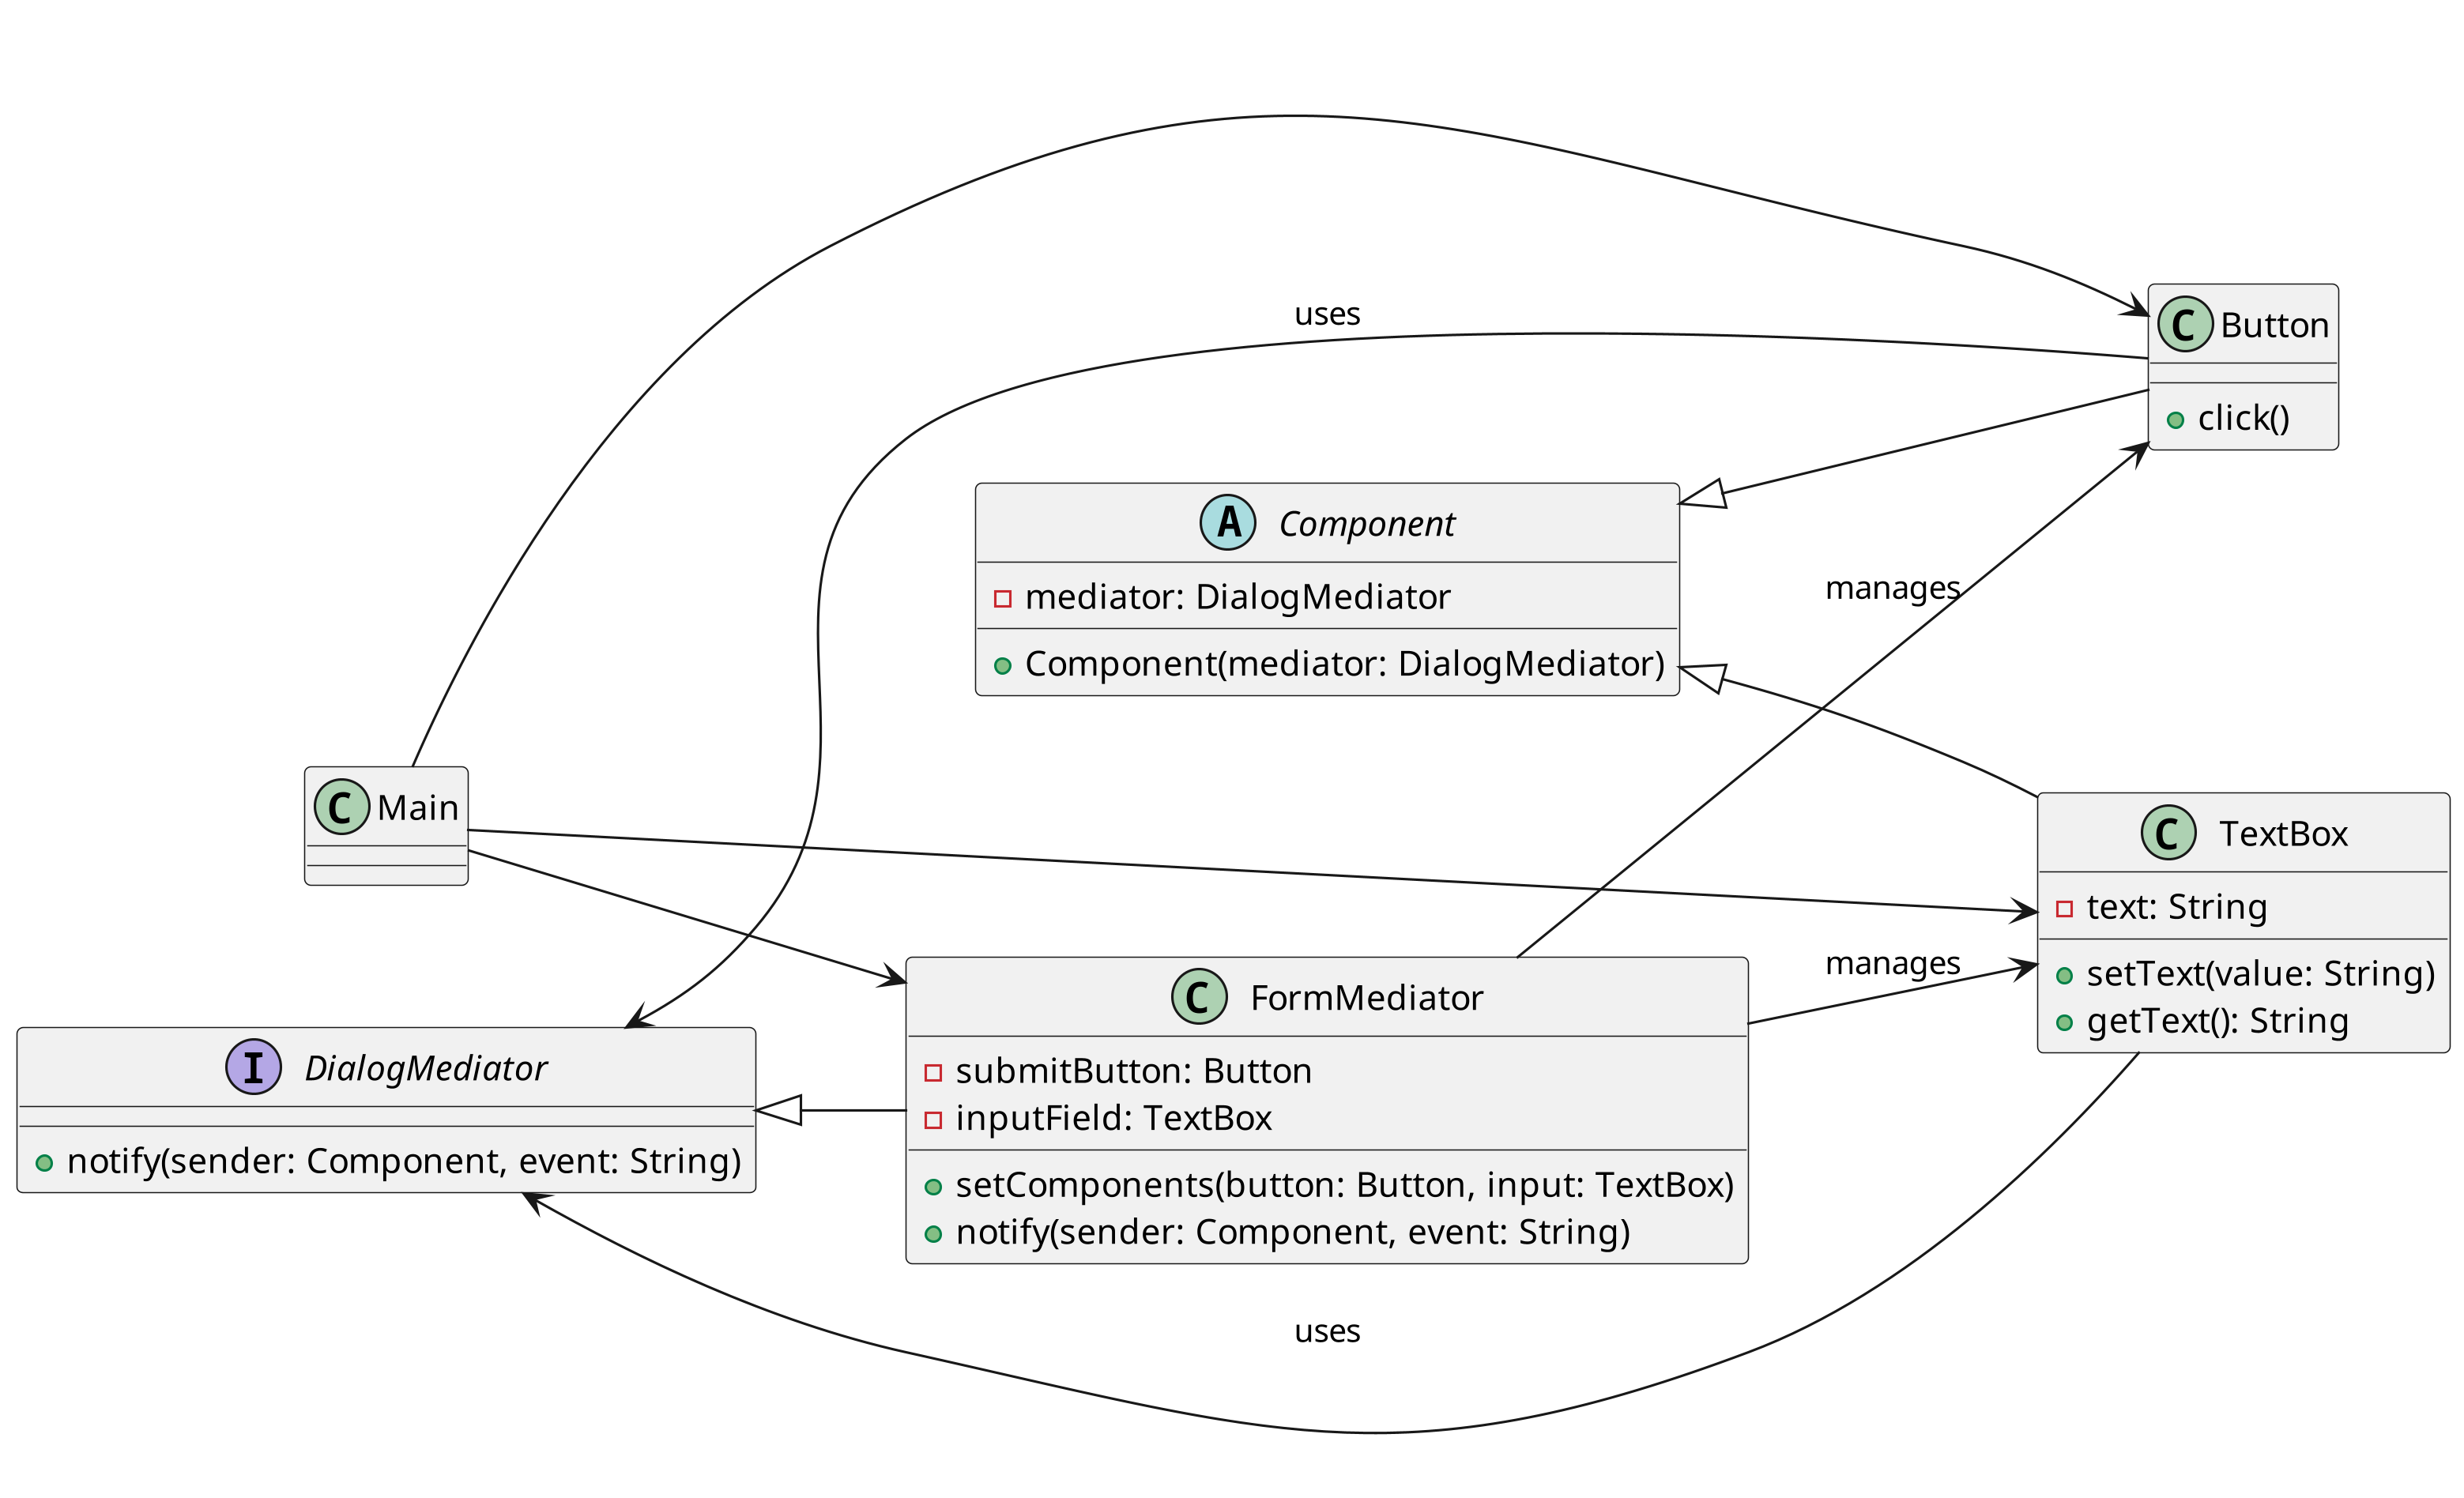
\includegraphics[width=0.8\textwidth]{../../figures/out/mediator.png}
\end{frame}

\begin{frame}[fragile]{Antarmuka Mediator dan Komponen Dasar}
\begin{lstlisting}[style=JavaStyle]
public interface DialogMediator {
	void notify(Component sender, String event);
}
\end{lstlisting}

\begin{lstlisting}[style=JavaStyle]
public abstract class Component {
	protected DialogMediator mediator;
	
	public Component(DialogMediator mediator) {
		this.mediator = mediator;
	}
}
\end{lstlisting}

\small Antarmuka \texttt{DialogMediator} mendefinisikan cara komunikasi antar komponen. Semua komponen menyimpan referensi ke mediator dan tidak saling mengenal langsung.
\end{frame}

\begin{frame}[fragile]{Komponen TextBox dan Button}
	\vspace{20pt}
\begin{columns}[t]
\column{0.55\textwidth}
\begin{lstlisting}[style=JavaStyle]
public class TextBox extends Component {
	private String text;
	public TextBox(DialogMediator mediator) {
		super(mediator);
	}
	public void setText(String value) {
		this.text = value;
		mediator.notify(this, "textChanged");
	}
	public String getText() {
		return text;
	}
}
\end{lstlisting}

\column{0.45\textwidth}
\begin{lstlisting}[style=JavaStyle]
public class Button extends Component {
	public Button(DialogMediator mediator) {
		super(mediator);
	}
	public void click() {
		mediator.notify(this, "click");
	}
}
\end{lstlisting}
\end{columns}

\small Kedua komponen tidak saling mengenal secara langsung, hanya berinteraksi lewat \texttt{mediator}.
\end{frame}


\begin{frame}[fragile]{Mediator Konkret: FormMediator}
	\vspace{20pt}
\begin{lstlisting}[style=JavaStyle]
public class FormMediator implements DialogMediator {
	private Button submitButton;
	private TextBox inputField;
	public void setComponents(Button button, TextBox input) {
		this.submitButton = button;
		this.inputField = input;
	}
	@Override
	public void notify(Component sender, String event) {
		if (sender == inputField && event.equals("textChanged")) {
			System.out.println("Input field changed: " + inputField.getText());
		} else if (sender == submitButton && event.equals("click")) {
			System.out.println("Submitting form with: " + inputField.getText());
		}
	}
}
\end{lstlisting}

\small \texttt{FormMediator} menangani semua logika interaksi berdasarkan event dan pengirimnya.
\end{frame}

\begin{frame}[fragile]{Client: Main}
\begin{lstlisting}[style=JavaStyle]
public class Main {
	public static void main(String[] args) {
		FormMediator mediator = new FormMediator();
		
		TextBox input = new TextBox(mediator);
		Button button = new Button(mediator);
		
		mediator.setComponents(button, input);
		
		input.setText("Hello Mediator!");
		button.click();
	}
}
\end{lstlisting}

\small Kelas \texttt{Main} menghubungkan semua komponen dengan mediator, lalu menjalankan interaksi.
\end{frame}

\section{Pola State}
\begin{frame}{\hfill}
\centering
\textbf{\Huge{Pola State}}
\end{frame}

\begin{frame}{State: Tujuan dan Konteks Penggunaan}
	\vspace{6pt}
	Pola \textit{State} memungkinkan objek mengubah perilaku saat status berubah. Setiap status diwakili kelas tersendiri, membuat sistem lebih modular, terstruktur, dan mudah diuji.
	
	\vspace{6pt}
	\begin{columns}[T]
		\column{0.48\textwidth}
		\textbf{Tujuan:}
		\begin{itemize}
			\item Hindari \texttt{if-else} kompleks.
			\item Pisahkan logika per status.
			\item Tambah status tanpa ubah kelas utama.
		\end{itemize}
		
		\textbf{Kapan Digunakan:}
		\begin{itemize}
			\item Perilaku tergantung status.
			\item Butuh transisi status eksplisit.
			\item Struktur kondisi sulit dikelola.
		\end{itemize}
		
		\column{0.48\textwidth}
		\textbf{Contoh:}
		\begin{itemize}
			\item \texttt{Dokumen:} Draft → Approved.
			\item \texttt{Vending Machine:} Idle → Dispensing.
			\item \texttt{Game:} Idle, Attack, Dead.
			\item \texttt{Koneksi:} Connected, Retry.
		\end{itemize}
	\end{columns}
\end{frame}


\begin{frame}{State: Contoh Kasus Penggunaan}
	\vspace{6pt}
	Pola \textit{State} cocok untuk sistem di mana status internal memengaruhi perilaku objek. Setiap status dibuat sebagai kelas terpisah untuk menjaga logika tetap modular dan mudah diuji serta dikembangkan.
	
	\vspace{6pt}
	\begin{itemize}
		\item \textbf{Vending Machine:} Status \texttt{Idle}, \texttt{HasMoney}, \texttt{Dispensing} menangani input berbeda.
		\item \textbf{Workflow Dokumen:} Transisi \texttt{Draft} → \texttt{Submitted} → \texttt{Approved}/\texttt{Rejected}.
		\item \textbf{Game Character:} Status seperti \texttt{Idle}, \texttt{Attacking}, \texttt{Dead} menentukan aksi dan animasi.
		\item \textbf{Network:} Status \texttt{Connecting}, \texttt{Connected}, \texttt{Reconnecting} mengatur event jaringan.
		\item \textbf{ATM:} Status \texttt{NoCard}, \texttt{HasCard}, \texttt{Authenticated} batasi aksi berdasarkan tahapan.
		\item \textbf{UI Form:} Status \texttt{Empty}, \texttt{Complete}, \texttt{Submitted} atur validasi dan navigasi.
	\end{itemize}
\end{frame}


\begin{frame}{State: Kelebihan dan Kekurangan}
\vspace{10pt}
Pola \textit{State} memisahkan perilaku berdasarkan status objek, membuat sistem lebih modular dan mudah dikembangkan. Namun, pola ini juga menambah kompleksitas desain.

\vspace{6pt}
\begin{columns}[T]
\column{0.5\textwidth}
\textbf{Kelebihan:}
\begin{itemize}
	\item Pisahkan logika berdasarkan status.
	\item Hindari \texttt{if-else}/\texttt{switch} kompleks.
	\item Tambah/ubah status tanpa ganggu kode lain.
	\item Transisi status eksplisit dan terkontrol.
	\item Modular dan mudah diuji.
\end{itemize}

\column{0.5\textwidth}
\textbf{Kekurangan:}
\begin{itemize}
	\item Jumlah kelas bisa membengkak.
	\item Transisi sulit dilacak tanpa dokumentasi.
	\item Butuh pemetaan transisi yang jelas.
	\item Tidak efisien untuk sistem sederhana.
	\item Berbagi data antar status bisa rumit.
\end{itemize}
\end{columns}

\vspace{4pt}
\small Cocok untuk sistem dengan status dinamis dan kompleks. Perlu pertimbangan skala agar tidak menambah beban desain.
\end{frame}

\begin{frame}{State: Struktur}
\centering
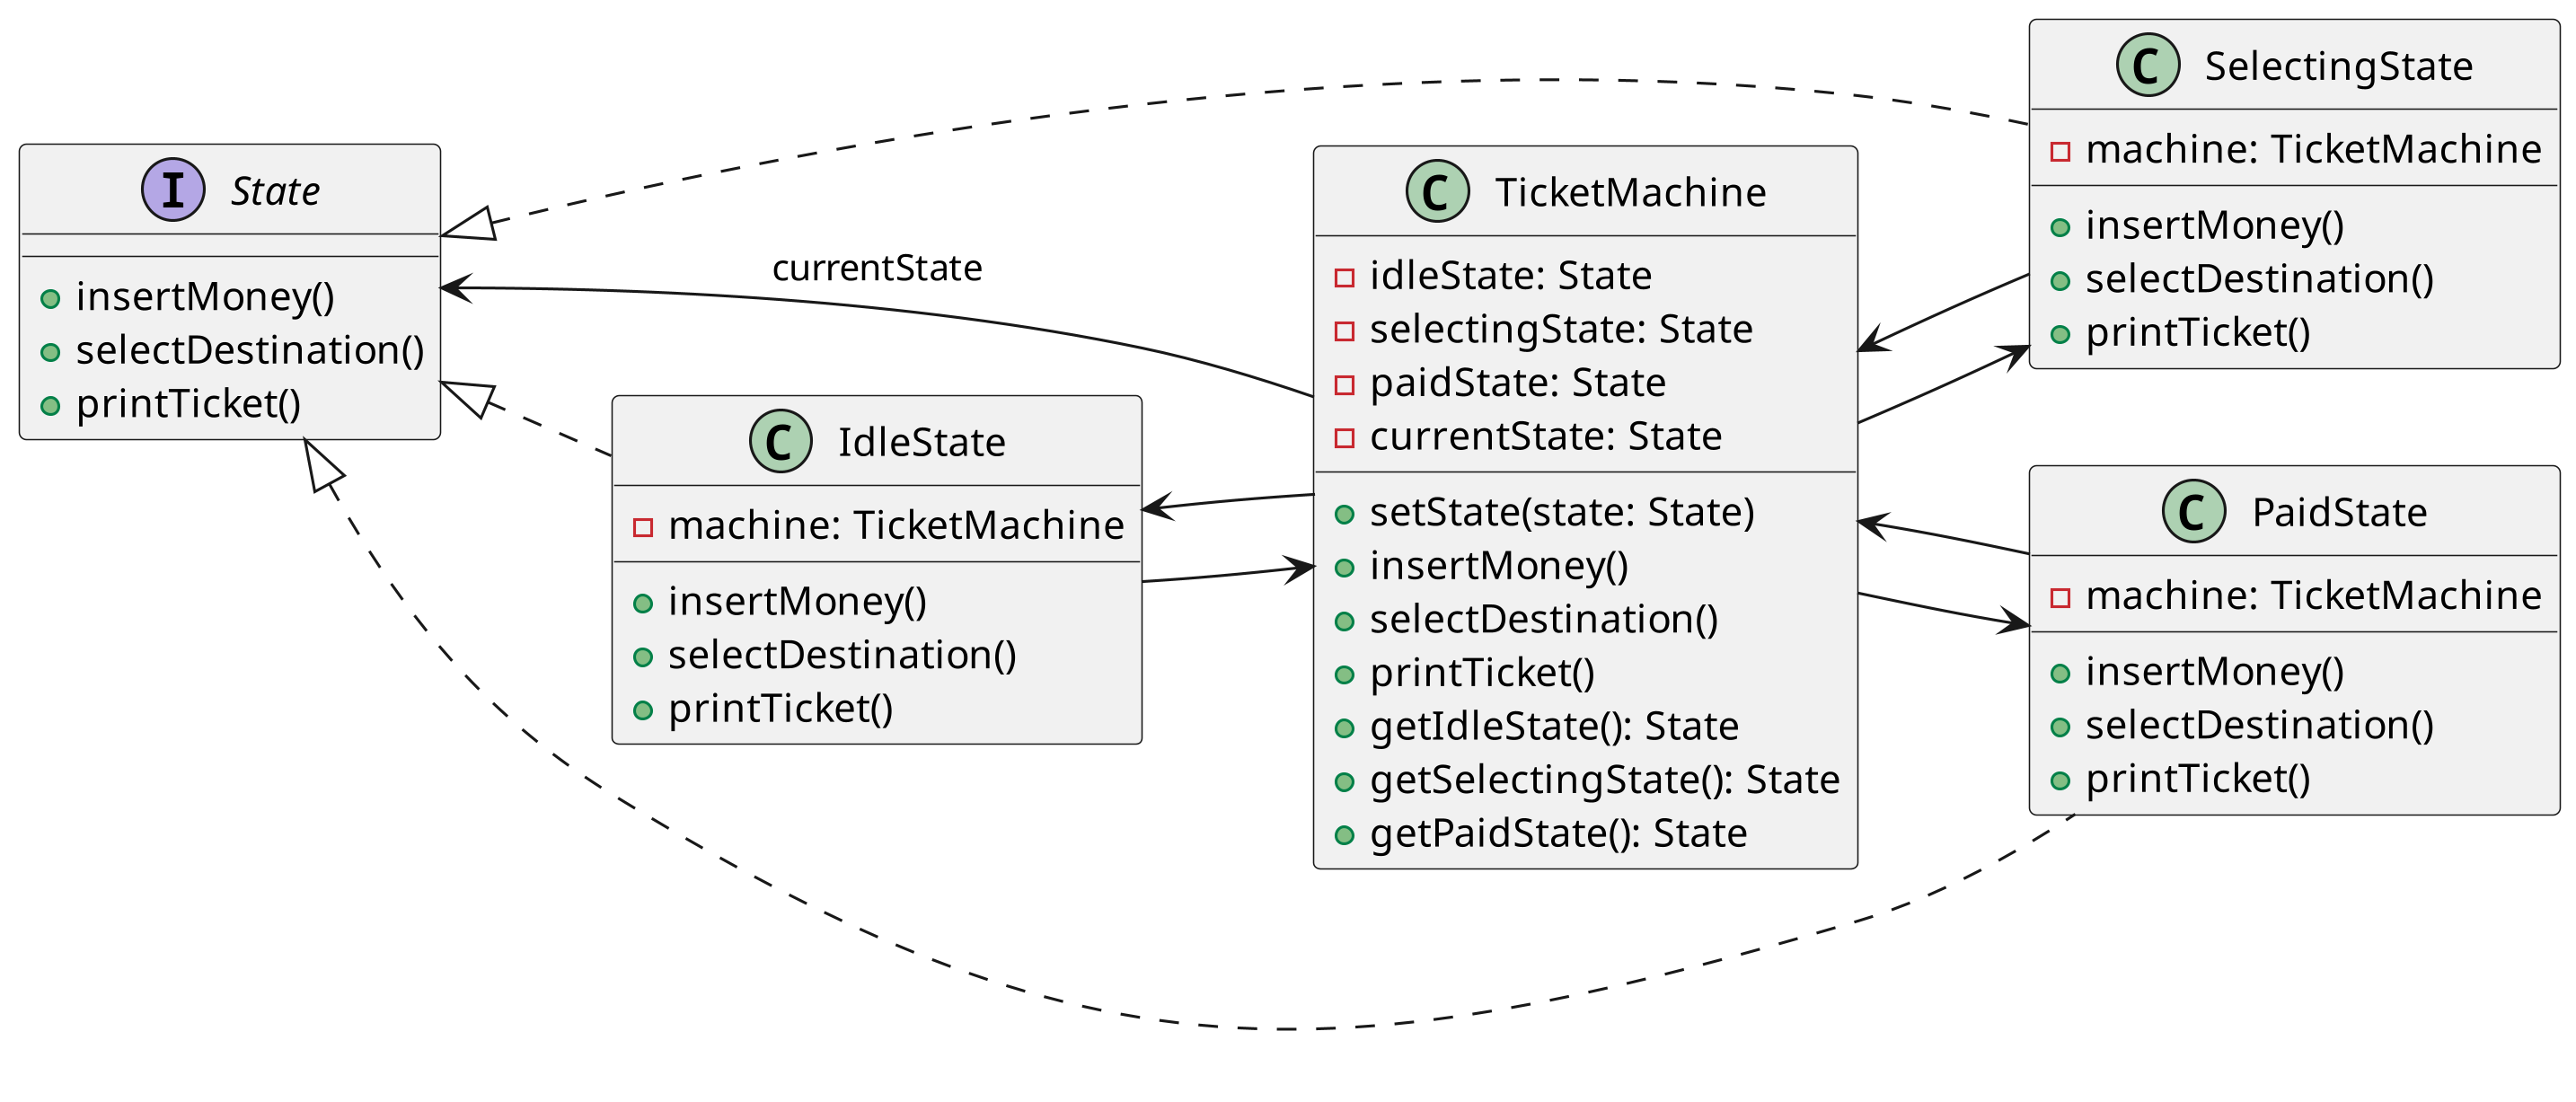
\includegraphics[width=0.85\textwidth]{../../figures/out/state.png}
\end{frame}

\begin{frame}[fragile]{State: Antarmuka}

\vspace{8pt}
\begin{lstlisting}[style=JavaStyle]
public interface State {
	void insertMoney();
	void selectDestination();
	void printTicket();
}
\end{lstlisting}

\small Antarmuka \texttt{State} mendefinisikan perilaku dasar semua status.
\end{frame}

\begin{frame}[fragile]{State: Implementasi IdleState}
	\vspace{20pt}
\begin{lstlisting}[style=JavaStyle]
public class IdleState implements State {
	private TicketMachine machine;
	public IdleState(TicketMachine machine) {
		this.machine = machine;
	}
	public void insertMoney() {
		System.out.println("Uang diterima.");
		machine.setState(machine.getSelectingState());
	}
	public void selectDestination() {
		System.out.println("Masukkan uang terlebih dahulu.");
	}
	public void printTicket() {
		System.out.println("Pilih tujuan terlebih dahulu.");
	}
}
\end{lstlisting}

\small \texttt{IdleState} hanya menerima uang dan berpindah ke \texttt{SelectingState}.
\end{frame}

\begin{frame}[fragile]{State: Context TicketMachine}
	\vspace{10pt}
\begin{columns}[T]
\column{0.5\textwidth}
\begin{lstlisting}[style=JavaStyle]
public class TicketMachine {
	private State idleState;
	private State selectingState;
	private State paidState;
	private State currentState;
	public TicketMachine() {
		idleState = new IdleState(this);
		selectingState = new SelectingState(this);
		paidState = new PaidState(this);
		currentState = idleState;
	}
	public void setState(State state) {
		this.currentState = state;
	}
	public void insertMoney() {
		currentState.insertMoney();
	}
\end{lstlisting}

\column{0.5\textwidth}
\begin{lstlisting}[style=JavaStyle]
	public void selectDestination() {
		currentState.selectDestination();
	}
	public void printTicket() {
		currentState.printTicket();
	}
	public State getIdleState() {
		return idleState;
	}
	public State getSelectingState() {
		return selectingState;
	}
	public State getPaidState() {
		return paidState;
	}
}
\end{lstlisting}
\end{columns}
\small \texttt{TicketMachine} menyimpan dan mendelegasikan aksi ke status aktif.
\end{frame}



\section{Pola Chain of Responsibility}
\begin{frame}{\hfill}
\centering
\textbf{\Huge{Pola Chain of Responsibility}}
\end{frame}


\begin{frame}{Tujuan dan Konteks Penggunaan}
	\vspace{10pt}
	\textit{Chain of Responsibility} memisahkan pengirim dan penerima permintaan dengan meneruskannya lewat rantai objek. Tiap handler memutuskan apakah menangani atau meneruskan.
	\begin{columns}[T]
		\column{0.5\textwidth}
		\textbf{Tujuan:}
		\begin{itemize}
			\item Hindari keterikatan langsung.
			\item Kurangi \texttt{if-else} kompleks.
			\item Urutan handler mudah diubah.
		\end{itemize}
		
		\textbf{Struktur:}
		\begin{itemize}
			\item \textbf{Handler:} Antarmuka umum.
			\item \textbf{ConcreteHandler:} Tangani atau teruskan.
			\item \textbf{Client:} Kirim permintaan ke awal rantai.
		\end{itemize}
		
		\column{0.5\textwidth}
		\textbf{Kapan Digunakan:}
		\begin{itemize}
			\item Permintaan bisa ditangani lebih dari satu objek.
			\item Klien tidak tahu siapa penerimanya.
			\item Handler bisa ditambah tanpa ubah klien.
		\end{itemize}
		
		\textbf{Contoh:}
		\begin{itemize}
			\item Validasi bertingkat, Logging bertahap, Approval multi-level, Middleware web.
		\end{itemize}
	\end{columns}
\end{frame}



\begin{frame}{Contoh Kasus Penggunaan}
	\vspace{10pt}
	Pola \textit{Chain of Responsibility} cocok untuk sistem di mana lebih dari satu objek bisa menangani permintaan secara berlapis dan fleksibel.
	
	\vspace{6pt}
	\begin{itemize}
		\item \textbf{Middleware Web:} Autentikasi dan logging diproses berurutan di Spring, Express, atau Phoenix.
		\item \textbf{Logging:} Pesan log ditangani sesuai level (\texttt{DEBUG}, \texttt{INFO}, \texttt{ERROR}).
		\item \textbf{Approval:} Permintaan diproses berjenjang: supervisor → manajer → direktur.
		\item \textbf{Validasi Form:} Email, password, dan konfirmasi dicek oleh validator berurutan.
		\item \textbf{Chatbot:} Tiap topik (lokasi, harga, jadwal) ditangani oleh handler khusus.
		\item \textbf{Error Handling:} Error ditangani handler sesuai jenis: parsing, jaringan, database.
	\end{itemize}
	
	\vspace{4pt}
	Pola ini menyederhanakan logika bercabang dan mendukung urutan proses yang dapat diatur ulang.
\end{frame}


\begin{frame}{Kelebihan dan Kekurangan}
	\vspace{10pt}
	Pola \textit{Chain of Responsibility} fleksibel untuk sistem berlapis, namun tetap memiliki keterbatasan desain.
	
	\vspace{4pt}
	\begin{columns}[T]
		\column{0.5\textwidth}
		\textbf{Kelebihan:}
		\begin{itemize}
			\item Handler baru mudah ditambah (Open/Closed).
			\item Loose coupling antara pengirim dan penerima.
			\item Tanggung jawab tiap handler lebih jelas.
			\item Urutan handler bisa diubah dinamis.
			\item Minim logika \texttt{if-else}.
		\end{itemize}
		
		\column{0.5\textwidth}
		\textbf{Kekurangan:}
		\begin{itemize}
			\item Sulit lacak siapa yang menangani.
			\item Debugging lebih kompleks.
			\item Overhead saat rantai panjang.
			\item Potensi ketergantungan antar handler.
			\item Permintaan bisa terhenti diam-diam.
		\end{itemize}
	\end{columns}
\end{frame}


\begin{frame}{Struktur Chain of Responsibility}
\centering
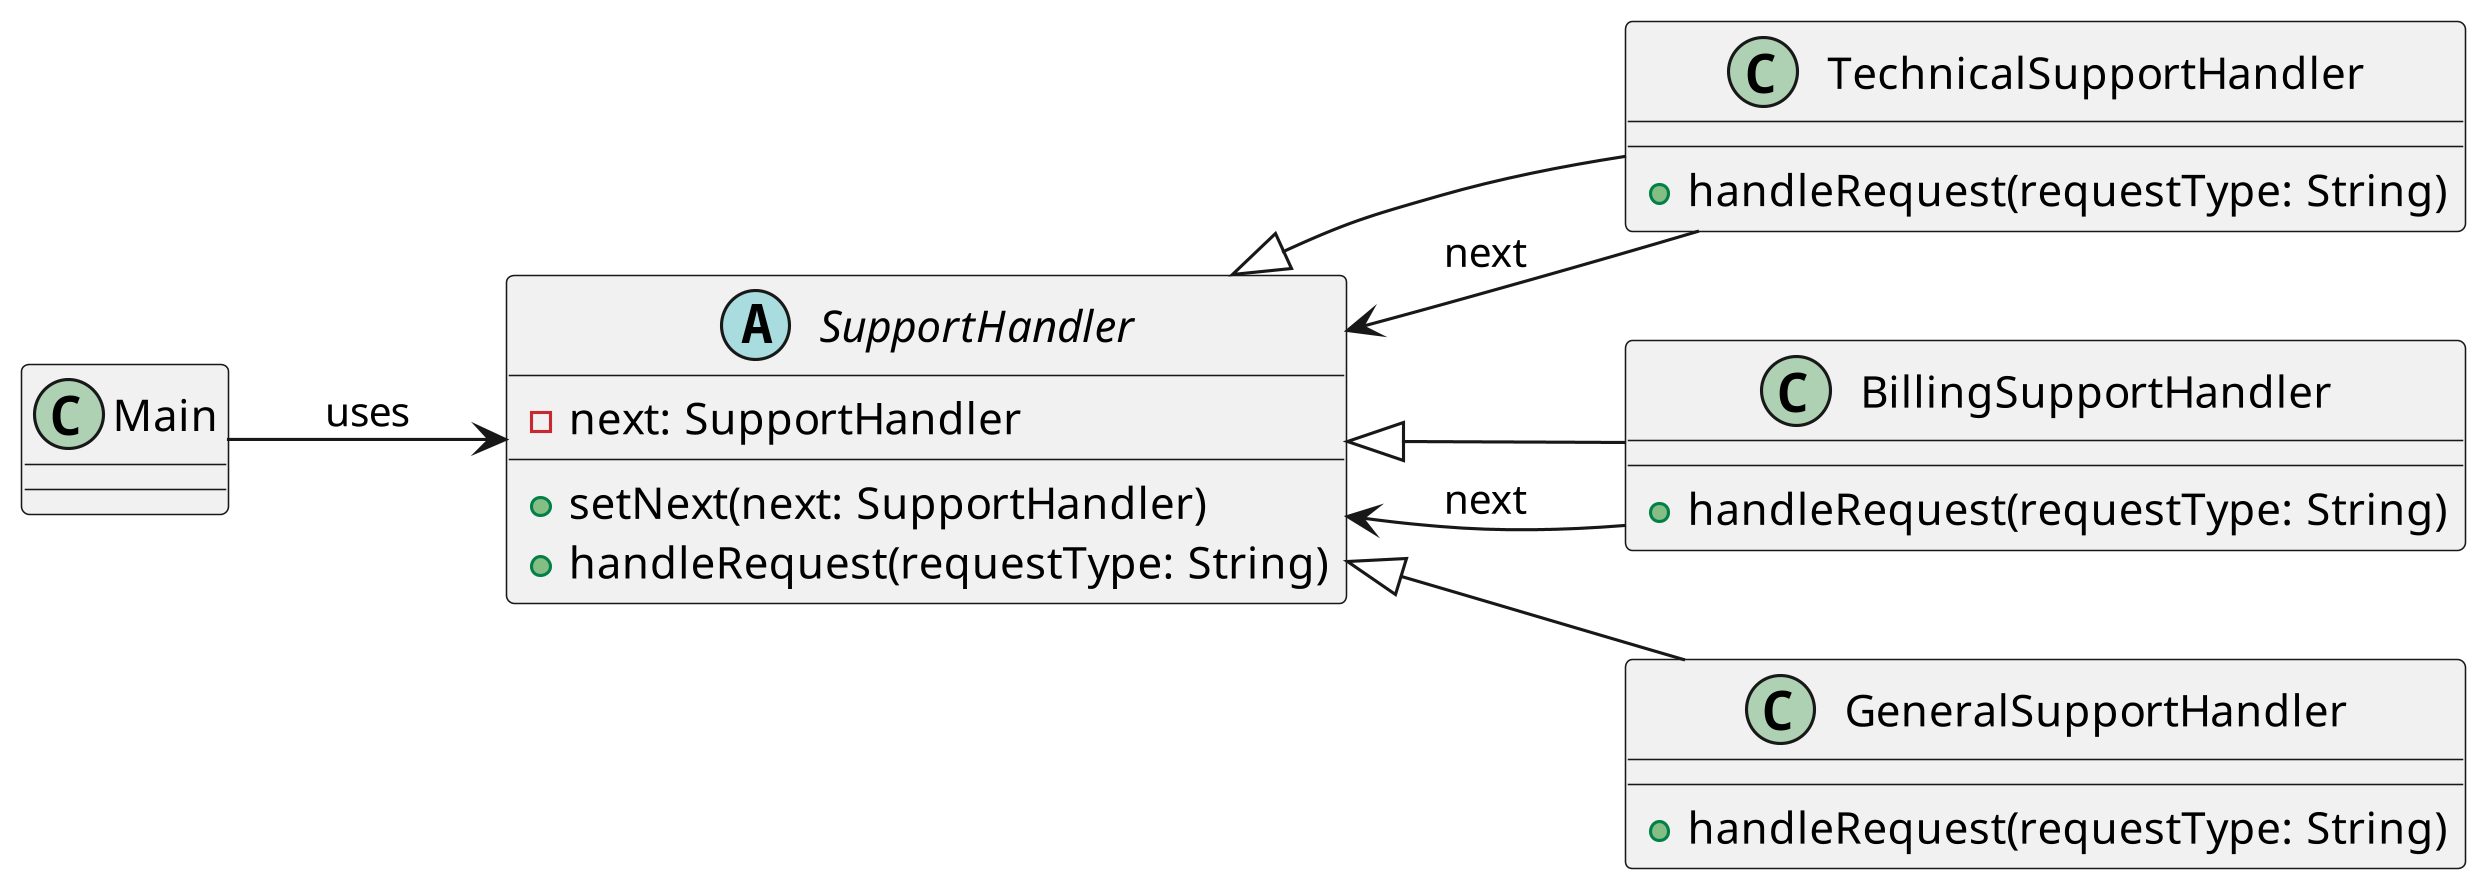
\includegraphics[width=\textwidth]{../../figures/out/chain_of_responsibility.png}
\vspace{4pt}
\small Struktur dasar terdiri dari \texttt{Handler}, \texttt{ConcreteHandler}, dan \texttt{Client} yang membentuk rantai pemrosesan.
\end{frame}

\begin{frame}[fragile]{Antarmuka Handler}
\begin{lstlisting}[style=JavaStyle]
public abstract class SupportHandler {
	protected SupportHandler next;
	
	public void setNext(SupportHandler next) {
		this.next = next;
	}
	
	public abstract void handleRequest(String requestType);
}
\end{lstlisting}
\small Kelas abstrak \texttt{SupportHandler} mendefinisikan kontrak dan rantai handler berikutnya.
\end{frame}

\begin{frame}[fragile]{Handler untuk Permintaan Teknis}
\begin{lstlisting}[style=JavaStyle]
public class TechnicalSupportHandler extends SupportHandler {
	@Override
	public void handleRequest(String requestType) {
		if ("Technical".equalsIgnoreCase(requestType)) {
			System.out.println("Ditangani oleh tim teknis.");
		} else if (next != null) {
			next.handleRequest(requestType);
		}
	}
}
\end{lstlisting}
\small Handler ini memproses permintaan teknis atau meneruskannya jika tidak sesuai.
\end{frame}

\begin{frame}[fragile]{Handler untuk Permintaan Penagihan}
\begin{lstlisting}[style=JavaStyle]
public class BillingSupportHandler extends SupportHandler {
	@Override
	public void handleRequest(String requestType) {
		if ("Billing".equalsIgnoreCase(requestType)) {
			System.out.println("Ditangani oleh tim penagihan.");
		} else if (next != null) {
			next.handleRequest(requestType);
		}
	}
}
\end{lstlisting}
\small Handler ini bertanggung jawab untuk menangani permintaan terkait penagihan.
\end{frame}

\begin{frame}[fragile]{Handler Default}
\begin{lstlisting}[style=JavaStyle]
public class GeneralSupportHandler extends SupportHandler {
	@Override
	public void handleRequest(String requestType) {
		System.out.println("Ditangani oleh tim umum.");
	}
}
\end{lstlisting}
\small Handler ini menangani permintaan umum yang tidak cocok dengan handler sebelumnya.
\end{frame}

\begin{frame}[fragile]{Client: Membentuk Rantai}
\begin{lstlisting}[style=JavaStyle]
public class Main {
	public static void main(String[] args) {
		SupportHandler tech = new TechnicalSupportHandler();
		SupportHandler billing = new BillingSupportHandler();
		SupportHandler general = new GeneralSupportHandler();
		
		tech.setNext(billing);
		billing.setNext(general);
		
		tech.handleRequest("Billing");
		tech.handleRequest("Technical");
		tech.handleRequest("Feedback");
	}
}
\end{lstlisting}
\small Klien membentuk rantai handler dan mengirimkan permintaan melalui handler pertama.
\end{frame}

\section{Pola Template Method}
\begin{frame}{\hfill}
\centering
\textbf{\Huge{Pola Template Method}}
\end{frame}

\begin{frame}{Tujuan dan Konteks Penggunaan}
	\vspace{10pt}
	Pola \textit{Template Method} mendefinisikan kerangka algoritma di superclass, sementara subclass menentukan detail langkah-langkah tertentu tanpa mengubah struktur utama.
	
	\vspace{6pt}
	\begin{columns}[T]
		\column{0.5\textwidth}
		\textbf{Tujuan:}
		\begin{itemize}
			\item Alur proses dipusatkan di superclass.
			\item Memisahkan bagian tetap dan yang bisa diubah.
			\item Menghindari duplikasi proses.
		\end{itemize}
		
		\textbf{Struktur:}
		\begin{itemize}
			\item \textbf{AbstractClass:} Template method.
			\item \textbf{ConcreteClass:} Override langkah.
		\end{itemize}
		
		\column{0.5\textwidth}
		\textbf{Kapan Digunakan:}
		\begin{itemize}
			\item Urutan proses tetap, detail fleksibel.
			\item Ingin alur dikendalikan oleh superclass.
			\item Cocok untuk workflow dan pipeline.
		\end{itemize}
		
		\textbf{Prinsip:}
		\begin{itemize}
			\item \textit{Hollywood Principle}: "Don't call us, we'll call you."
		\end{itemize}
	\end{columns}
\end{frame}


\begin{frame}{Template Method: Contoh Kasus Penggunaan}
	\vspace{10pt}
	Pola \textit{Template Method} digunakan untuk proses yang terstruktur namun tetap memungkinkan variasi di langkah-langkah tertentu. Contoh:
	
	\vspace{2pt}
	\begin{itemize}
		\item \textbf{Login/Autentikasi:} Alur login tetap, mekanisme autentikasi disesuaikan di subclass (password, OTP, OAuth).
		\item \textbf{Workflow Dokumen:} Alur approval konsisten, detail langkah sesuai tipe dokumen.
		\item \textbf{Siklus Game Loop:} Urutan update–logic–render ditetapkan superclass; detail disesuaikan subclass.
		\item \textbf{Ekspor Laporan:} Proses ekspor sama, format file ditentukan subclass (PDF, Excel, CSV).
		\item \textbf{Unit Test Framework:} Struktur test tersedia di superclass; isi test di subclass.
		\item \textbf{Transaksi Pembayaran:} Langkah validasi hingga eksekusi tetap; metode bayar fleksibel.
	\end{itemize}
\end{frame}


\begin{frame}{Template Method: Kelebihan dan Kekurangan}
	\vspace{10pt}
	Pola \textit{Template Method} cocok untuk sistem dengan proses tetap namun langkah-langkah yang bervariasi. Berikut kelebihan dan kekurangannya:
	
	\vspace{6pt}
	\begin{columns}[T]
		\column{0.5\textwidth}
		\textbf{Kelebihan:}
		\begin{itemize}
			\item Reuse struktur algoritma di superclass.
			\item Subclass fokus pada detail langkah.
			\item Perubahan cukup di superclass.
			\item Cocok untuk framework/library.
			\item Tambah perilaku tanpa modifikasi.
		\end{itemize}
		
		\column{0.5\textwidth}
		\textbf{Kekurangan:}
		\begin{itemize}
			\item Ketergantungan subclass pada superclass.
			\item Hierarki dalam menyulitkan debugging.
			\item Tidak fleksibel untuk runtime switch.
			\item Subclass bisa isi metode kosong.
			\item Tidak ideal untuk proses dinamis.
		\end{itemize}
	\end{columns}
\end{frame}



\begin{frame}[fragile]{Template Method: Struktur Pola}
	\vspace{20pt}
\centering
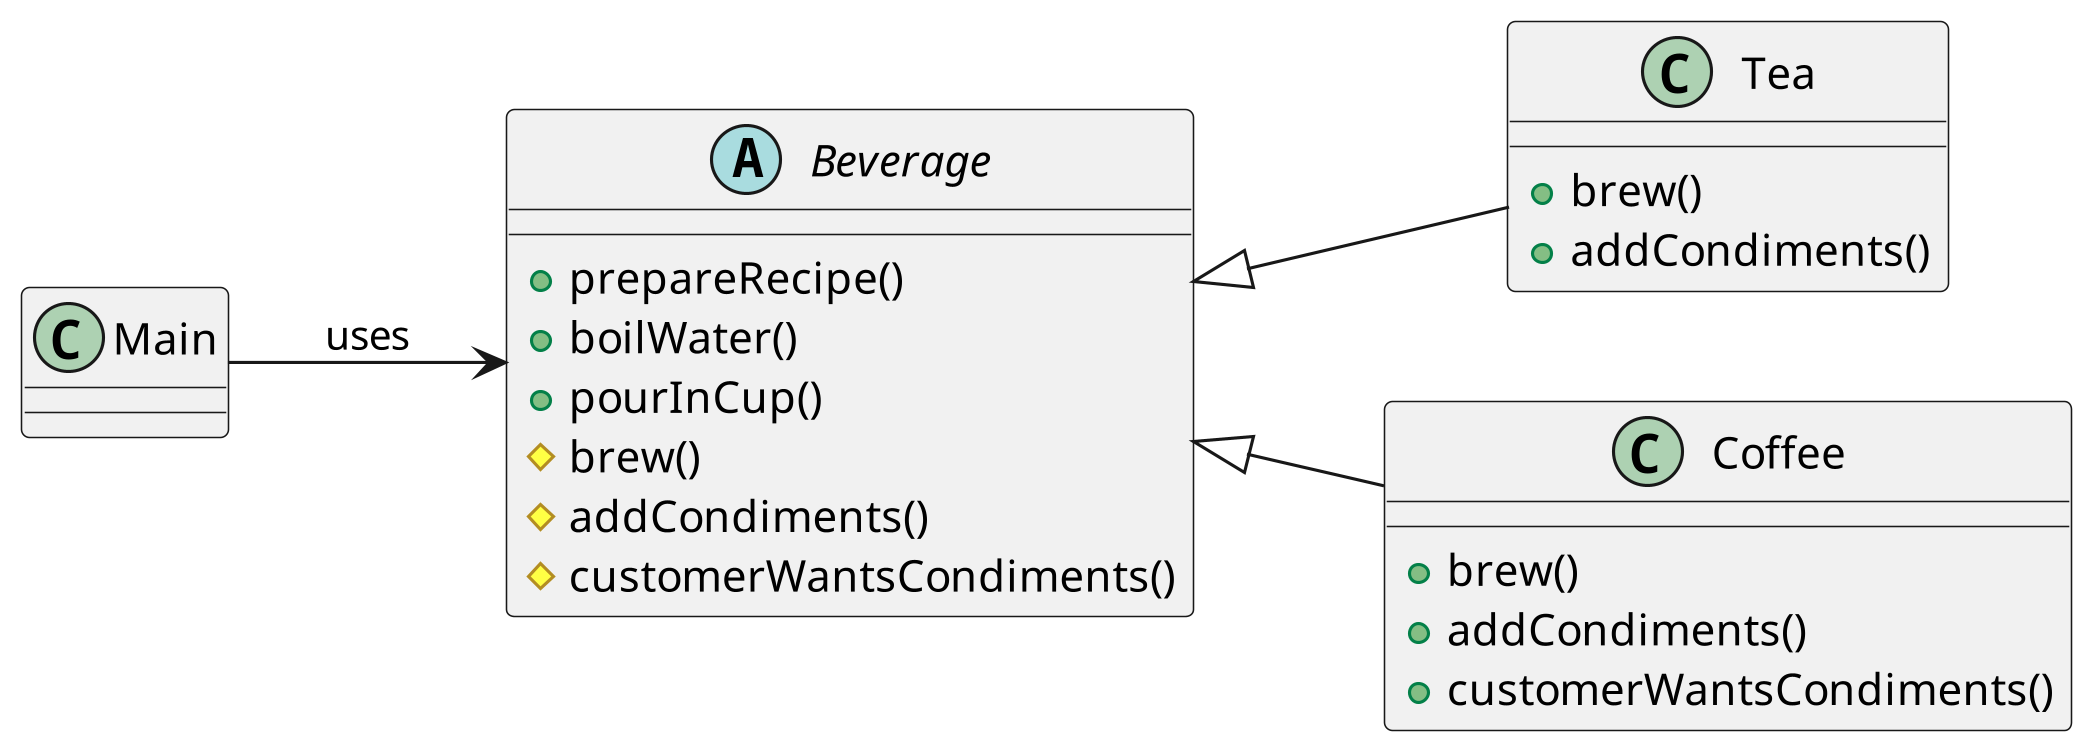
\includegraphics[width=0.9\textwidth]{../../figures/out/template_method.png}
\vspace{6pt}
\small Struktur umum Template Method terdiri dari kelas abstrak yang mendefinisikan kerangka proses dan subclass yang mengisi langkah-langkah detail.
\end{frame}

\begin{frame}[fragile]{Template Method: AbstractClass}
\begin{columns}[t]
\column{0.5\textwidth}
\begin{lstlisting}[style=JavaStyle]
public abstract class Beverage {
	public final void prepareRecipe() {
		boilWater();
		brew();
		pourInCup();
		if (customerWantsCondiments()) {
			addCondiments();
		}
	}
	protected void boilWater() {
		System.out.println("Boiling water");
	}
\end{lstlisting}

\column{0.5\textwidth}
\begin{lstlisting}[style=JavaStyle]
	protected void pourInCup() {
		System.out.println("Pouring into cup");
	}
	protected abstract void brew();
	protected abstract void addCondiments();
	
	protected boolean customerWantsCondiments() {
		return true;
	}
}
\end{lstlisting}
\end{columns}

\vspace{4pt}
	\small Kelas \texttt{Beverage} mendefinisikan urutan langkah tetap dengan metode template \texttt{prepareRecipe()}.
\end{frame}


\begin{frame}[fragile]{Template Method: Subclass untuk Teh}
\begin{lstlisting}[style=JavaStyle]
public class Tea extends Beverage {
	@Override
	protected void brew() {
		System.out.println("Steeping the tea");
	}
	@Override
	protected void addCondiments() {
		System.out.println("Adding lemon");
	}
}
\end{lstlisting}
\vspace{4pt}
\small Kelas \texttt{Tea} mengisi langkah penyeduhan dan tambahan sesuai jenis minuman.
\end{frame}

\begin{frame}[fragile]{Template Method: Subclass untuk Kopi}
\begin{lstlisting}[style=JavaStyle]
public class Coffee extends Beverage {
	@Override
	protected void brew() {
		System.out.println("Dripping coffee through filter");
	}
	@Override
	protected void addCondiments() {
		System.out.println("Adding sugar and milk");
	}
	@Override
	protected boolean customerWantsCondiments() {
		return false; // tanpa tambahan
	}
}
\end{lstlisting}
\vspace{4pt}
\small Kelas \texttt{Coffee} mengoverride \texttt{hook method} untuk menonaktifkan tambahan.
\end{frame}

\begin{frame}[fragile]{Template Method: Client Code}
\begin{lstlisting}[style=JavaStyle]
public class Main {
	public static void main(String[] args) {
		Beverage tea = new Tea();
		tea.prepareRecipe();
		
		System.out.println();
		
		Beverage coffee = new Coffee();
		coffee.prepareRecipe();
	}
}
\end{lstlisting}
\vspace{4pt}
\small Kode klien menggunakan template method tanpa mengetahui detail langkah yang diimplementasikan oleh subclass.
\end{frame}


\begin{frame}{Kesimpulan: Pola Perilaku Lanjutan}
	\vspace{10pt}
	Empat pola perilaku lanjutan memberikan struktur yang efisien untuk sistem perangkat lunak kompleks:
	
	\vspace{6pt}
	\begin{itemize}
		\item \textbf{Mediator:} Memusatkan komunikasi objek untuk mengurangi keterikatan dan menyederhanakan interaksi.
		
		\item \textbf{State:} Mengubah perilaku objek berdasarkan status internal secara modular dan fleksibel.
		
		\item \textbf{Chain of Responsibility:} Menyusun handler dalam rantai dinamis untuk validasi, middleware, atau approval.
		
		\item \textbf{Template Method:} Menetapkan urutan tetap dan mengizinkan subclass menyesuaikan langkah tertentu.
	\end{itemize}
	
	\vspace{6pt}
	\small Penerapan pola ini mendukung desain modular dan mudah diperluas. Pilih sesuai kebutuhan, kompleksitas, dan alur logika sistem.
\end{frame}







\end{document}
